\section{Planification}
\todoWho{Matt}

\todoGeneric{3 à 5 pages de planification}

\subsection{Fonctionnalités}

Le robot est un lanceur de balle de bière-pong qui a comme utilisation première de lancer des balles dans des verres.
Le robot sera contrôlé par un utilisateur à l’aide d’une application mobile qui lui permettra de le faire bouger de gauche à droite et de contrôler la force du moteur avec de lancer la balle.
De plus, des verres intelligents accompagne le robot.
Les verres capte les détectes les balles à l’intérieur du verre pour avertir au joueur quels verres sont réussis à l’aide de lumières qui s’allument.

\subsection{Planification}

\todo{Planification et suivi de projet}

\todoDoing{Listes des fonctionnalités du produit avec modifications (Gantt).}

Au début du projet, nous avons identifié plusieurs fonctionnalité d'un produit final.
Pour plusieurs de ces fonctionnalités, nous avons jugé que certaines n'étaient pas nécessaires pour un prototype.

\begin{enumerate}
    \item Lance avec précision
    \item Joue des chansons
    \item Danse/Célèbre la victoire de l’équipe du propriétaire
    \item Se déplace et lance automatiquement ou manuellement à l’aide d’une manette contrôlé par un humain
    \item Communique avec les verres pour savoir si le lancer est réussi ou non
    \item Écœure l’autre équipe (joue la chanson sad violon quand ils manquent les verres)
    \item Contrôlable pour viser les joueurs de l’autre équipe
\end{enumerate}

\begin{figure}[h!]
    \centering
    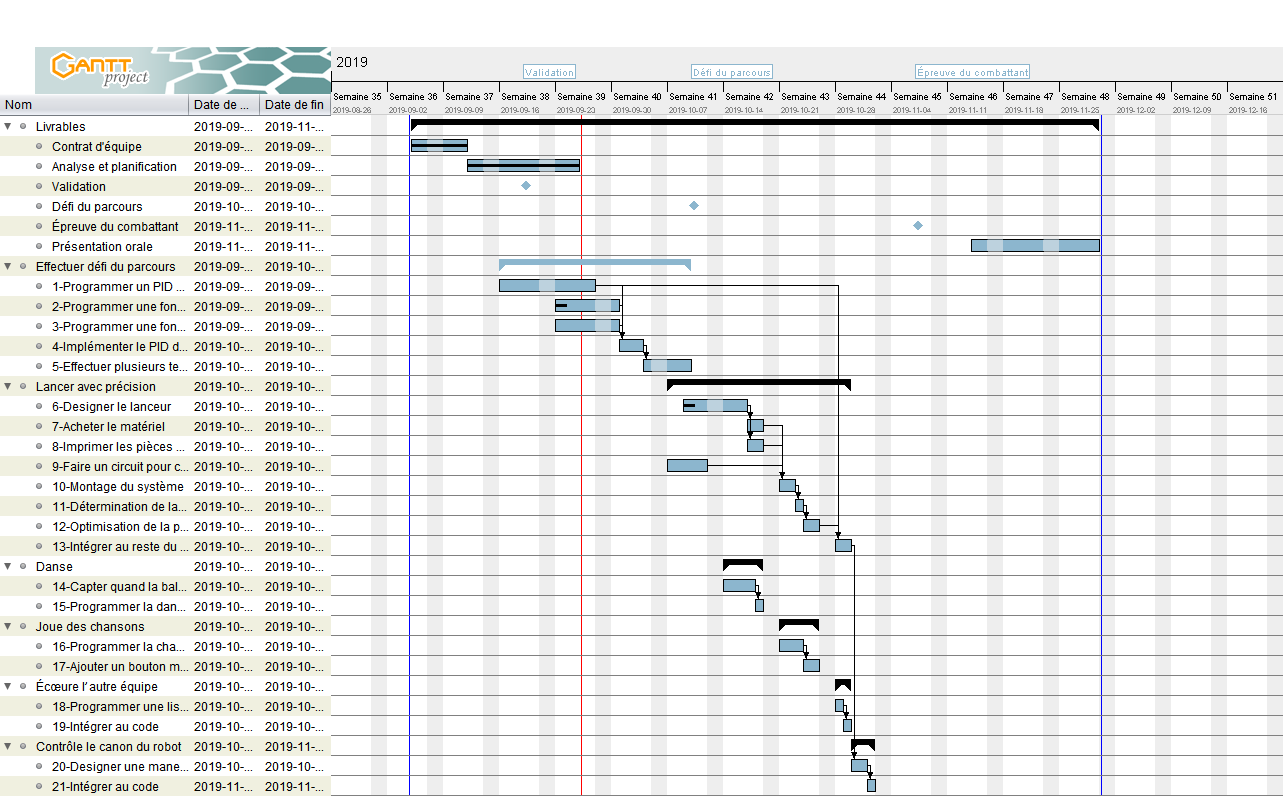
\includegraphics[width=\linewidth]{img/s1/robuck-2019-09-26}
    \caption{Diagramme de Gantt intial}
    \label{fig:planif-initial}
\end{figure}

\todoPoints{Listes des fonctionnalités du produit avec modifications (Gantt).}

\subsection{Gestion du projet et outils}


Des tâches ont été ajouté en cours de projet.

Nous avons pris la décision de retirer certaines tâches dont nous jugions moins pertinente.
\todo{Ajouter exemples de tâches supprimé}
Nous avons tenu des réunions hebdomadaires de suivis.
Ces rencontres nous ont permis d'ajuster la distribution hebdomadaires des tâches.

Nous avons utilisé le service Trello en tant que tableau de bord afin de nous aider à prioriser les tâches.

\begin{figure}[h!]
    \centering
    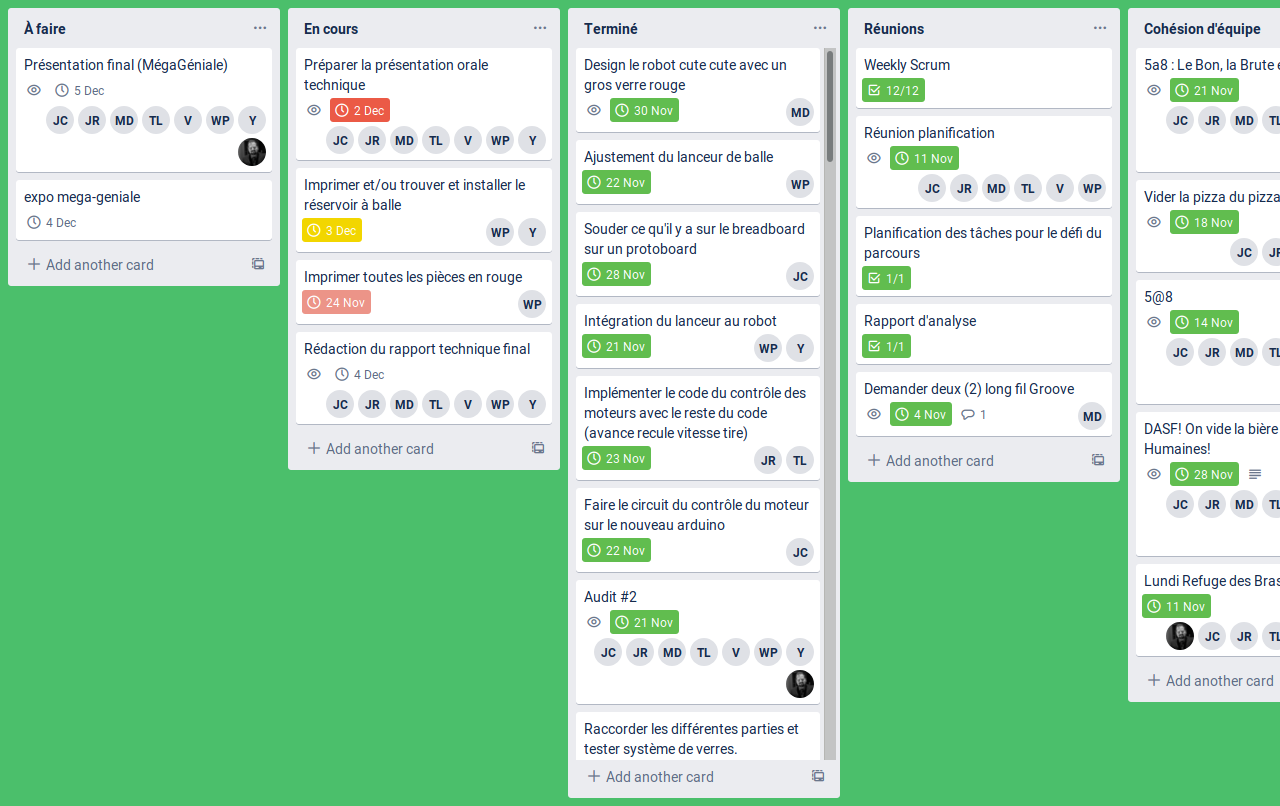
\includegraphics[width=\linewidth]{img/s1/trello}
    \caption{Implémentation d'un Kanban à l'aide de Trello}
    \label{fig:planif-trello}
\end{figure}
